\documentclass[11pt]{article}
\usepackage{graphics,epsfig,amsmath,amssymb}
\usepackage{epsf}
\usepackage{boxedminipage}
\usepackage{fullpage}
\usepackage{fancyheadings}
\usepackage{times}
\usepackage{amsmath}
\usepackage{ifthen}
\usepackage{pseudocode}
\usepackage{psfrag}
\pagestyle{fancy}

\setlength{\topmargin}{.2in}
\setlength{\parindent}{0in}
\setlength{\parskip}{.15in}
\setlength{\footskip}{0.1in}

\newcounter{pctr}
\stepcounter{pctr}

\newcounter{partctr}

\newcommand{\ie}{{\em i.e.}}
\newcommand{\eg}{{\em e.g.}}

\newcommand{\ch}{\item {\bf True~~/~~False~~}}
\newcommand{\tfnote}{\probnote{Circle True or False for each choice.}}
\newcommand{\allapply}{\probnote{Circle ALL that apply}}
\newcommand{\bestanswer}{\probnote{Circle the BEST answer}}
\newcommand{\ansbelow}{\probnote{Answer legibly in the space below.}}

\renewcommand{\thesection}{{\bf\Roman{section}}}
\renewcommand{\theenumi}{{\bf\Alph{enumi}.}}
\renewcommand{\labelenumi}{{\bf\Alph{enumi}.}}

\newcommand{\setversion}[1]{\def\version{#1}}
\setversion{quiz}

\ifthenelse{\equal{\version}{answers}}{
    \newcommand{\sols}[1]{#1}
} {
    \newcommand{\sols}[1]{}
}


\newcounter{answer}
\newenvironment{answer}[1][\relax]{\refstepcounter{answer}\begin{list}%
 {}{\leftmargin 0pt\rightmargin 0pt\labelsep 3pt\parsep 0pt%
 \setlength{\listparindent}{\parindent}}
    \item {\bf Answer \theanswer #1}\
    }{\hspace*{\fill}$\blacksquare$\end{list}} 



% uses these macros to delimit problems
\newcommand\prob[1]%
  {\begin{itemize}\item[]%
   \vspace{.2in}{\bf\thepctr. ~[#1~ points]:}\stepcounter{pctr}}
\newcommand\eprob{\end{itemize}}
\newcommand\probnote[1]%
  {\\\begin{tabular}{cr} \hspace{3in} & {\bf (#1)} \\ \end{tabular}}

% headers/footers
\lhead[\fancyplain{}{\bf Page \thepage ~of \pageref{lastpage}}]%
      {CS 3251 Spring 2013, Quiz 1}
\lfoot[{\bf Initials: }]%
      {{\bf Initials: }}
\rhead[CS 3251 Spring 2013, Quiz 1]%
      {\fancyplain{}{\bf Page \thepage ~of \pageref{lastpage}}}
\cfoot{}
\setlength{\headrulewidth}{0in}
\setlength{\headsep}{.3in}

 % Compact itemize and enumerate.  Note that they use the same counters and
% symbols as the usual itemize and enumerate environments.
\def\compactify{\itemsep=0pt \topsep=0pt \partopsep=0pt \parsep=0pt}
\let\latexusecounter=\usecounter
\newenvironment{CompactItemize}
  {\def\usecounter{\compactify\latexusecounter}
   \begin{itemize}}
  {\end{itemize}\let\usecounter=\latexusecounter}
\newenvironment{CompactEnumerate}
  {\def\usecounter{\compactify\latexusecounter}
   \begin{enumerate}}
  {\end{enumerate}\let\usecounter=\latexusecounter}

\begin{document}
\cfoot{}
\pagestyle{empty}
\begin{center}
\begin{tabular}{lr}
\resizebox{1in}{!}{\includegraphics{GT}}
&
\parbox{4in}{
    {\Large\it College of Computing} \\ \\
    {\LARGE\sf Georgia Institute of Technology} 
}
%
\end{tabular}
\end{center}

\begin{center}
{\Large{\bf CS 3251: Computer Networking: Spring 2013} \\
 \vspace{.15in} \Huge{\bf Quiz I}} 
\vspace{.2in}

% this is the box on the first page with overall quiz information
\begin{boxedminipage}[h]{6in}
There are \underline{12 questions} and \underline{\pageref{lastpage}
  pages} in this quiz booklet (including this page), plus one optional
bonus question. {\bf There are 90 total points.}  Answer each question according to the instructions
given.  You have {\bf 85 minutes} to answer the questions.

\vspace{.1in} The last page is an easy, optional set of questions.  {\em
  Rip this page off of your exam for five bonus points.}  Turn it in
anonymously.


\vspace{.1in} 
If you find a question ambiguous, write down any
assumptions you make.  {\bf Be neat and legible.}  If I can't
understand your answer, I can't give you credit!  
%There are three pretty
%challenging questions (clearly marked); you may want to look through the
%whole quiz and save those for last.

\vspace{.1in} 
Use the empty sides of this booklet if you need scratch space.  You
may also use them for answers, although you shouldn't need to.  {\em If you
do use the blank sides for answers, make sure to clearly say so!}

\vspace{.1in} 
{\bf Note well: Write your name in the space below AND your initials at the bottom of each
page of this booklet.}

\begin{center}{\bf THIS IS AN ``CLOSED BOOK'' QUIZ.\\
NO BOOKS, NO NOTES, NO OTHER MATERIALS, NO PHONES, NO COMPUTERS, NO
LAPTOPS, NO PDAS.\\ 
ONE TWO-SIDED LETTER-SIZED NOTE SHEET IS ALLOWED.
%NO ENCRYPTED WIRELESS TRAFFIC. \\
MAKE SURE YOU'VE READ ALL THE INSTRUCTIONS ABOVE!}
\end{center}
{\em Initial here to indicate that (1)~you've read the instructions and (2)~
you agree to abide by the Georgia Tech Honor Code: }



\if 0
\vspace{.05in} The last page has easy bonus questions, {\em which you can
answer outside of the allotted time}.  Rip the last page off of your
quiz for five bonus points.  Turn it in anonymously if you like (feel
free to fill it out after the quiz and give it to a TA, or take it with you).  You
won't get the five points if you don't tear off the page (this is to
make certain you've read this far ;).
\fi 

\end{boxedminipage}
\end{center}
\vspace*{0.15in}
\begin{center}
{\it Do not write in the boxes below}
\end{center}

\begin{center}
\begin{tabular}{|l|l|l|l|l|l|l|l|l|} \hline \hline
{\bf 1-5 (xx/20)}& {\bf 6-8 (xx/24)} & {\bf 9 (xx/14)} & {\bf 10-11
  (xx/20)} & {\bf 12 (xx/12)} &{\bf Bonus (xx+5)} & {\bf Total
  (xx/90)}  \\ \hline 
 & & & & & & \\ 
 & & & & & & \\ \hline \hline
\end{tabular}
\end{center}

\vspace{.1in}
{\bf\Large{Name:}}

\newpage
\pagestyle{fancy}

\section{Warmup}



\prob{4} 
Which of the following are true about Classless Interdomain Routing (CIDR)?
\allapply

\setcounter{partctr}{0}
\begin{list}{\bf\Alph{partctr}.}{\usecounter{partctr}}
\item The prefix length for a CIDR prefix can be anywhere in the range from 0 to 32
  bits.
\item CIDR slowed the rate of Internet routing table growth because
  prefixes no longer had to be allocated in fixed-size blocks.
\item In an Internet forwarding table with CIDR, there can only be one
  unique matching entry for any given IP address.
\item The only sizes for an IP address allocation before CIDR were 8,
  16, or 24 bits.
\item All of the above.
\end{list}
\eprob

\sols{
\begin{answer}
The answer is: (A), (B), (D)
\end{answer}
}

\prob{4} 
Which of the following are true about how DNS lookups work?
\allapply

\setcounter{partctr}{0}
\begin{list}{\bf\Alph{partctr}.}{\usecounter{partctr}}
\item An MX-record query for a DNS lookup will return the IP address of
  the mail server for that domain.
\item An NS-record query for a DNS lookup will return the name(s) of the
  authoritative name server(s) for that domain.
\item A DNS A-record query for {\tt google.com} will only return a
  single IP address at a time.
\item All DNS PTR records are maintained by a single organization {\tt in-addr.arpa}.
\item If your local DNS resolver caches an NS record for {\tt
  google.com} for multiple days, all clients who use that DNS resolver
  will continue using the same IP address to reach Google's Web server
  until that NS record expires.
\end{list}
\eprob

\sols{
\begin{answer}
The answer is: (B)
\end{answer}
}

\newpage
\prob{4} 
Which of the following are true about traffic control with BGP?
\allapply

\setcounter{partctr}{0}
\begin{list}{\bf\Alph{partctr}.}{\usecounter{partctr}}
\item A network operator can use BGP {\em AS path prepending} to control
  {\em inbound} traffic from his or her AS to a destination.
\item A network operator can use the BGP {\em local preference} attribute to
  control {\em inbound} traffic from his or her AS to a destination.
\item A network operator can use BGP {\em AS path prepending} to control
  {\em outbound} traffic from his or her AS to a destination.
\item A network operator can use the BGP {\em local preference} attribute to
  control {\em outbound} traffic from his or her AS to a destination.
\item All of the above.
\end{list}
\eprob

\sols{
\begin{answer}
The answer is: (A), (D).
\end{answer}
}



\prob{4} 
Which of the following are true about layering?
\allapply

\setcounter{partctr}{0}
\begin{list}{\bf\Alph{partctr}.}{\usecounter{partctr}}
\item The transport layer uses port numbers.
\item The network layer guarantees reliable, in-order delivery of
  packets.
\item The network layer has only a single protocol in widespread use
  today, representing what we call the ``narrow waist''.
\item The destination address in the link layer header is
  always the address of the next layer-3 node along an end-to-end IP
  path.
\item All of the above.
\end{list}
\eprob

\sols{
\begin{answer}
The answer is (A), (C), (D).
\end{answer}
}


\prob{4} 
Which of the following are true about packet switching?
\allapply

\setcounter{partctr}{0}
\begin{list}{\bf\Alph{partctr}.}{\usecounter{partctr}}
\item A user of a packet-switched network might occasionally get a
  ``busy signal'' if there are too many users on the network.
\item Traffic running over a packet-switched network between two endpoints will always
  experience predictable latency.
\item Traffic running over a packet-switched network between two
  endpoints will never be dropped by intermediate nodes along the path.
\item Once a connection is established between two endpoints in a packet
  switched network, the end-to-end route cannot change, or the
  connection must be re-established.
\item All of the above.
\end{list}
\eprob

\sols{
\begin{answer}
The answer is: (B), (C).
\end{answer}
}




%%%%%%%%%%%%%%%%%%%%%%%%%%%%%%%%%%%%%%%%%%%%%%%%%%%%%%%%%%%%

\newpage
\section{Routing and Addressing}

\prob{6} Describe two advantages of link-state routing over
distance-vector routing.  Describe one disadvantage.~\ansbelow
\vspace{1.75in}
\eprob

\sols{
\vspace{-1.75in}
\begin{answer}
\end{answer}
}

\prob{10}  Suppose that you have an IP address {\tt 18.31.132.110} and the
following prefixes in a forwarding table.  
\begin{center}
\begin{tabular}{r}
18.0.0.0/8 \\
18.31.0.0/16 \\
18.31.128.0/17 \\
18.31.128.0/24 \\
\end{tabular}
\end{center}
(a)~Which of the following prefixes in the Internet routing table will this prefix
match?  \\ (b)~How many IP addresses does each of these four IP prefixes represent?
~\ansbelow 
\vspace{1.25in}
\eprob

\sols{
\vspace{-1.25in}
\begin{answer}
\end{answer}
}
\newpage

\pagebreak
\prob{8} Consider the following traceroute from Georgia Tech to
BBC {\tt news.bbc.co.uk}.  Each row in the output below shows one IP
``hop'' along the path from Georgia Tech to {\tt news.bbc.co.uk}, along
with the round-trip latency to that hop in milliseconds (there are three
measurements of round-trip latency for each hop).
\begin{scriptsize}
\begin{verbatim}
% traceroute news.bbc.co.uk
traceroute to news.bbc.co.uk (212.58.246.84), 30 hops max, 60 byte packets
 1  cc-cisco-143out4.cc.gt.atl.ga.us (143.215.131.1)  1.255 ms  1.748 ms  1.099 ms
 2  ni-rtr-gorillanet.gatech.edu (130.207.251.1)  1.730 ms  1.710 ms  1.549 ms
 3  campus2-rtr-130-207-254-45.gatech.edu (130.207.254.45)  2.463 ms  2.463 ms  2.458 ms
 4  gateway2-rtr.gatech.edu (130.207.254.185)  2.010 ms  2.002 ms  1.975 ms
 5  atx-edge-04.inet.qwest.net (65.114.55.137)  47.960 ms  47.956 ms  47.931 ms
 6  atx-brdr-01.inet.qwest.net (67.14.14.138)  1.949 ms  1.362 ms  1.268 ms
 7  63.146.27.198 (63.146.27.198)  1.558 ms  1.849 ms  1.821 ms
 8  ash-bb3-link.telia.net (80.91.251.85)  16.709 ms 16.716 ms 15.520 ms
 9  ldn-bb2-link.telia.net (80.91.251.208)  91.007 ms 92.489 ms 90.481 ms
10  ldn-b3-link.telia.net (80.91.249.176)  89.620 ms 90.773 ms 90.458 ms
11  atos-ic-124708-ldn-b2.c.telia.net (213.248.104.70)  101.540 ms  100.094 ms  99.794 ms
12  * * *
13  * * *
14  ae0.er01.cwwtf.bbc.co.uk (132.185.254.93)  90.664 ms  95.325 ms  91.188 ms
15  132.185.255.165 (132.185.255.165)  95.860 ms  99.814 ms  99.818 ms
16  bbc-vip005.cwwtf.bbc.co.uk (212.58.246.84)  89.450 ms  90.388 ms  89.411 ms
\end{verbatim}
\end{scriptsize}
(a)~Which hop is the first hop on the {\em other side} of the Atlantic
Ocean?  Why? \\
(b)~How many autonomous systems (ASes) are likely on this path?  How did
you figure out your answer? \\
(c)~How does the {\tt traceroute} tool map from the IP addresses along
the path to provide human-readable names, as above? (A one-sentence
answer is sufficient here.) \\
(d)~Why is the last hop on the traceroute
``bbc-vip005.cwwtf.bbc.co.uk'', even though the IP address of the last
hop is {\tt 212.58.246.84}, which is the IP address for
``news.bbc.co.uk''?  (in other words, why do the names not match?)
\vspace{1.75in}
\eprob

\sols{
\vspace{-1.25in}
\begin{answer}
\end{answer}
}

\newpage
\section{Domain Name System}
\prob{14} Consider the following (abridged) ``dig'' trace.  Remember that the
``trace'' option forces an iterative lookup, even if certain DNS records
are cached in the local resolver.
\begin{scriptsize}
\begin{verbatim}
% dig nytimes.com +trace
; <<>> DiG 9.7.3 <<>> nytimes.com +trace
;; global options: +cmd
.			308148	IN	NS	b.root-servers.net.
.			308148	IN	NS	c.root-servers.net.
.			308148	IN	NS	d.root-servers.net.
.			308148	IN	NS	e.root-servers.net.
.			308148	IN	NS	a.root-servers.net.
;; Received 512 bytes from 130.207.17.21#53(130.207.17.21) in 2 ms

com.			172800	IN	NS	g.gtld-servers.net.
com.			172800	IN	NS	m.gtld-servers.net.
com.			172800	IN	NS	j.gtld-servers.net.
com.			172800	IN	NS	b.gtld-servers.net.
com.			172800	IN	NS	d.gtld-servers.net.
com.			172800	IN	NS	k.gtld-servers.net.
;; Received 489 bytes from 199.7.91.13#53(d.root-servers.net) in 40 ms

nytimes.com.		172800	IN	NS	dns.sea1.nytimes.com.
nytimes.com.		172800	IN	NS	dns.ewr1.nytimes.com.
;; Received 107 bytes from 192.48.79.30#53(j.gtld-servers.net) in 177 ms

nytimes.com.		500	IN	A	170.149.168.130
nytimes.com.		500	IN	A	170.149.172.130
;; Received 61 bytes from 170.149.173.133#53(dns.sea1.nytimes.com) in 96 ms
\end{verbatim}
\end{scriptsize}
(a)~Which of the records above were likely already in the local DNS
resolver's cache when this lookup was performed?  Explain how you
arrived at your answer. \\
(b)~Which of these DNS records will be kept in the local DNS resolver's
cache for the shortest amount of time?  How long will those records be
cached? \\
(c)~What are the authoritative DNS name servers for {\tt nytimes.com}?
\\
(d)~How much time did it take for the above DNS query to complete? Show
your work. \\
(e)~If a
regular A-record query
for {\tt nytimes.com} were run again immediately (without the ``trace'' option), about how long would you expect the
query to take? Why? 
 \ansbelow \eprob

\sols{
\begin{answer}
\end{answer}
}

\newpage
\section{Border Gateway Protocol}

\prob{10} Consider the autonomous system graph below.  Assume that a
directed edge represents a relationship from a customer to a provider,
and that an undirected edge represents a peering link.

\begin{center}
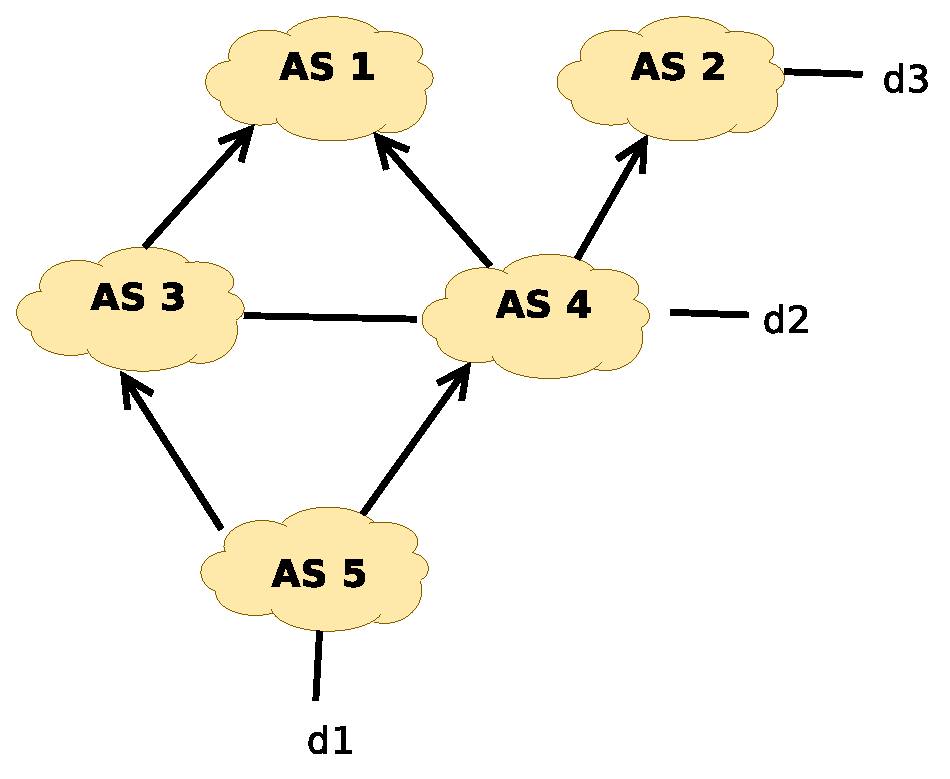
\includegraphics[width=0.4\linewidth]{as-rel}
\end{center}
(a)~Which ASes will learn at least one route to $d_1$? \\
(b)~Which ASes will learn at least one route to $d_2$? \\
(c)~Which ASes will learn at least one route to $d_3$? \\
(d)~Suppose that AS~3 learns a route to $d_1$ via AS~4 and AS~5.  Which
route will it prefer, and why?
~\ansbelow \eprob

\sols{
\begin{answer}
\end{answer}
}

\newpage
\prob{10} Consider the routing table dump excerpt for {\tt 1.0.0.0/24}.

\begin{scriptsize}
\begin{verbatim}
   Network          Next Hop             Local Preference AS Path
*  1.0.0.0/24       72.36.126.8          100              40387 2381 15169 
*                   202.147.61.12        90               10026 15169 
*                   218.189.6.129        80               9304 15169 
\end{verbatim}
\end{scriptsize}
(a)~Which route in the table above will be the preferred route?
\\ 
(b)~Based on the settings of local preference on the routes above and
the AS paths in the table, which ASes are likely the customer, peer, and
provider AS for the autonomous system where this routing table was
collected?  ~\ansbelow \eprob

\newpage
\section{Putting It All Together}

Consider the network diagram below.  Suppose that switches construct
layer 2 spanning  trees, and routers perform IP routing between networks
(both between subnets within an AS and between ASes).
\begin{center}
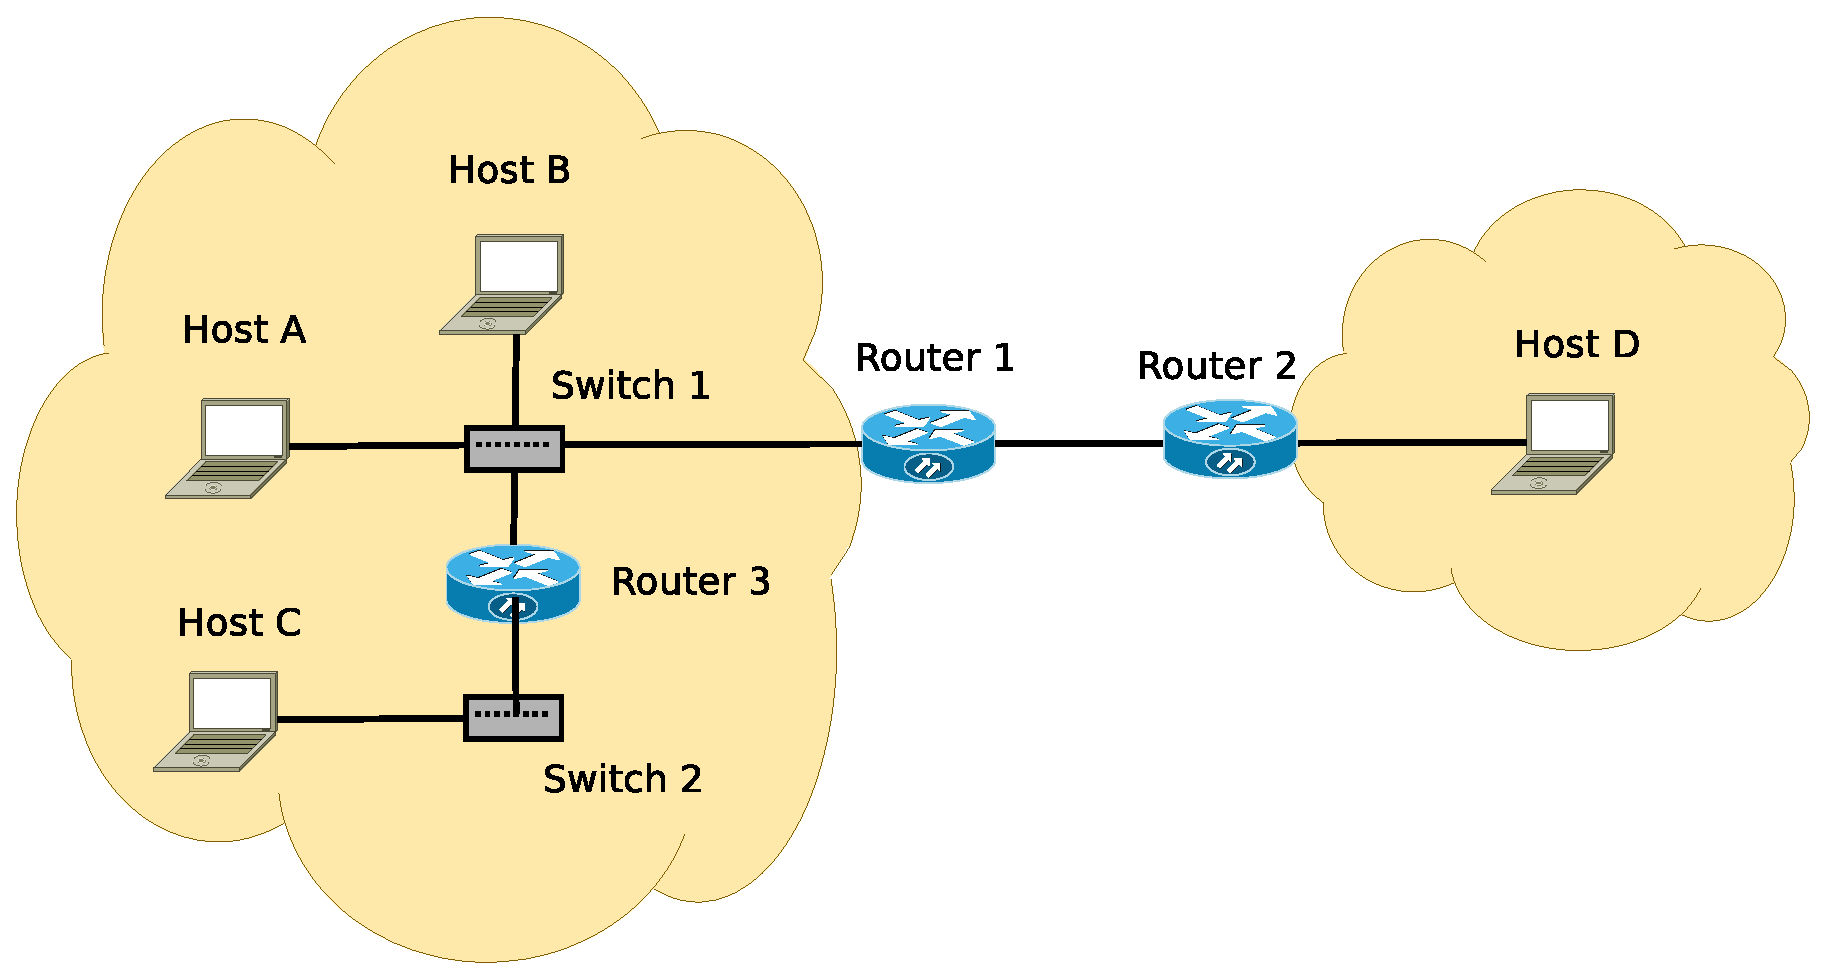
\includegraphics[width=0.65\linewidth]{network}
\end{center}



\prob{12} Suppose hosts A, B, C, and D have
all been sending traffic to each other continually for some time. \\
(a)~What nodes will have entries in Host A's ARP table? \\
(b)~What nodes will have entries in Switch 1's switch table? \\
(c)~What routing protocols will Host A use to construct a route to Host
B, if any? \\
(d)~What routing protocols will Host C use to construct a route to Host
B, if any? \\
(e)~What routing protocols will Host A use to construct a route to Host
D, if any? \\
\ansbelow
\eprob
\vspace*{1.25in}
\sols{
\vspace{-1.25in}

}


\newpage
\section{Bonus: Redesigning ARP}

\prob{5} {\bf Bonus Design Question! Optional!} George Burdell finds the
current ARP broadcast protocol incredibly wasteful as a lookup
protocol. ``A host has to broadcast to every other host on the network
to learn the MAC address for a single IP address. Why can't we just use
the DNS?''  Imagine you could put IP addresses into the DNS.  How might
you do it? ({\em hint:} Consider how reverse lookups work.)  How might
your design be similar or different from the way reverse DNS lookups
work to map IP addresses to domain names? (Consider things like TTL
values, whether you might need fewer or more ``authoritative servers'',
etc.) \\ \ansbelow \eprob
\vspace*{1.25in}
\sols{
\vspace{-1.25in}

}


\newpage
\section*{Anonymous Course Feedback}
{\bf This page is anonymous.}  Rip this off from your exam, and turn it
in separately if you like.  You'll get five points for simply ripping
off the last page of the exam, but I'd prefer if you fill it out and
hand it in in a separate stack.
\vspace{.5in}

What are the things you like most about the course so far?  Anything is
fair game here (topics, course structure, board technique, etc.).
\vspace{1.5in}


What are the things you like least about the course so far?  Again,
anything is fair game.
\vspace{1in}


What topics would you like to see covered?
\vspace{1in}



\label{lastpage}
\end{document}
